\subsection{Cấu trúc dữ liệu biểu diễn đồ thị}
\subsubsection{Thiết kế phần mềm}
\textit{Đồ thị các thành phần phụ thuộc (Module Dependency Graphs)} \\
Một trong những nhiệm vụ quan trọng trong thiết kế phần mềm đó là chia chương trình
thành nhiều thành phần hoặc module khác nhau để tiện cho việc phát triển mà mở rộng
cũng như bảo trì sau này. Việc hiểu được sự tương tác giữa các modules trong một 
chương trình tương tác với nhau như thế nào là cực kì quan trọng không chỉ trong việc 
thiết kế chương trình mà còn trong việc kiểm thử và bảo trì nữa. Một đồ thị các thành 
phần phụ thuộc giúp ích rất nhiều trong việc này. Trong đồ thị các thành phần phụ thuộc 
(dependencies), mỗi đỉnh biểu thị một module, một cạnh nối có hướng chỉ sự phụ thuộc 
của module này vào module kia. Một ví dụ về đồ thị biểu diễn sự phụ thuộc của các modules
trong một ứng dụng web: 
\begin{figure}[H] % places figure environment here   
    \centering % Centers Graphic
    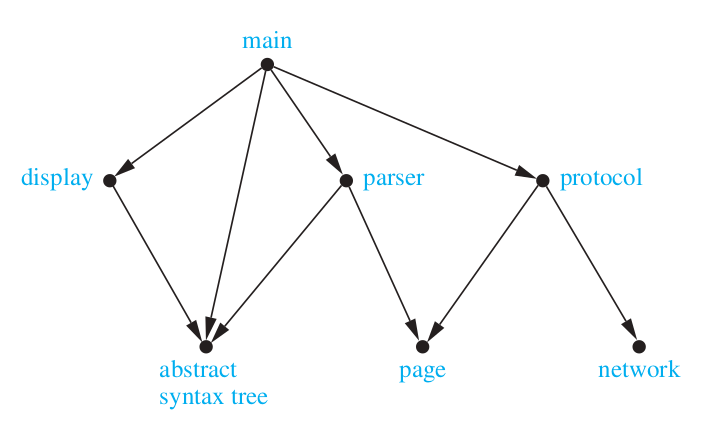
\includegraphics[width=0.6\textwidth]{assets/web_grp.png} 
    \caption{Ví dụ đồ thị sự phụ thuộc của các modules
    trong một ứng dụng web} % Creates caption underneath graph
    \label{fig:gr_1.2.1}
\end{figure}

\subsubsection{Mạng giao thông}
Mô hình đồ thị được sử dụng trong nhiều loại mạng giao thông khác nhau như đường bộ, 
hàng không, mạng đường sắt và mạng chuyển phát. \\

\textit{Định tuyến trong hàng không} \\
Mô hình mạng hàng không có thể được biểu diễn bằng đồ thị với mỗi sân bay là một đỉnh.
Các chuyến bay từ sân bay này tới sân bay khác có thể được biểu diễn bằng một cạnh 
có hướng từ sân bay cất cánh (đỉnh bắt đầu) đến sân bay hạ cánh (đỉnh kết thúc). \\

\textit{Mạng đường bộ} \\
Mô hình đồ thị có thế được sử dụng để biểu diễn mạng đường bộ mà trong đó các đỉnh 
thể hiện các giao lộ và các cạnh thể hiện đường đi. Khi tất cả các cong đường trong mạng 
đều là đường 2 chiều thì ta có thể biểu diễn mạng bằng một đơn đồ thị vô hướng. Tuy 
nhiên trong thực tế ta thường gặp trong mạng giao thông thì một số đường là 2 chiều
và một số khác là 1 chiều. Để biểu diễn mạng này ta dùng cạnh vô hướng để biểu diễn 
đường 2 chiều và cạnh có hướng để biểu diễn đường một chiều.

\subsubsection{Mạng sinh học}
\textit{Đồ thị chồng chéo ngách trong hệ sinh thái} \\
